\documentclass{sigchi}

% Remove or comment out these two lines for final version
\toappearbox{\Large Submitted to CHI'13. \\Do not cite, do not circulate.}
\pagenumbering{arabic}% Arabic page numbers for submission. 

% Use \toappear{...} to override the default ACM copyright statement (e.g. for preprints).

% Load basic packages
\usepackage{balance}  % to better equalize the last page
\usepackage{graphicx} % for EPS, load graphicx instead
\usepackage{times}    % comment if you want LaTeX's default font
\usepackage{url}      % llt: nicely formatted URLs
\usepackage{tabularx}
\usepackage{subfigure}
\usepackage[usenames,table]{xcolor}

% llt: Define a global style for URLs, rather that the default one
\makeatletter
\def\url@leostyle{%
  \@ifundefined{selectfont}{\def\UrlFont{\sf}}{\def\UrlFont{\small\bf\ttfamily}}}
\makeatother
\urlstyle{leo}


% To make various LaTeX processors do the right thing with page size.
\def\pprw{8.5in}
\def\pprh{11in}
\special{papersize=\pprw,\pprh}
\setlength{\paperwidth}{\pprw}
\setlength{\paperheight}{\pprh}
\setlength{\pdfpagewidth}{\pprw}
\setlength{\pdfpageheight}{\pprh}

% Make sure hyperref comes last of your loaded packages, 
% to give it a fighting chance of not being over-written, 
% since its job is to redefine many LaTeX commands.
\usepackage[pdftex]{hyperref}
\hypersetup{
pdftitle={SIGCHI Conference Proceedings Format},
pdfauthor={LaTeX},
pdfkeywords={SIGCHI, proceedings, archival format},
bookmarksnumbered,
pdfstartview={FitH},
colorlinks,
citecolor=black,
filecolor=black,
linkcolor=black,
urlcolor=black,
breaklinks=true,
}

% create a shortcut to typeset table headings
\newcommand\tabhead[1]{\small\textbf{#1}}


% End of preamble. Here it comes the document.
\begin{document}

\title{Touchscreen Keyboard Hierarchical Spatial Models with Back-offs for
Hand Posture and Personal Adaptation}

% Note that submissions are blind, so author information should be omitted
\numberofauthors{3}
\author{
  \alignauthor 1st Author Name\\
    \affaddr{Affiliation}\\
    \affaddr{Address}\\
    \email{e-mail address}\\
  \alignauthor 2nd Author Name\\
    \affaddr{Affiliation}\\
    \affaddr{Address}\\
    \email{e-mail address}\\
  \alignauthor 3rd Author Name\\
    \affaddr{Affiliation}\\
    \affaddr{Address}\\
    \email{e-mail address}\\
}

% Teaser figure can go here
%\teaser{
%  \centering
%  \includegraphics{Figure1}
%  \caption{Teaser Image}
%  \label{fig:teaser}
%}

\maketitle

\begin{abstract}
In this sample paper, Sheridan Printing Co., Inc. 
describe the formatting requirements for
SIGCHI Conference Proceedings, and this sample file
offers recommendations on writing for the worldwide
SIGCHI readership. Please review this document even if
you have submitted to SIGCHI conferences before, some
format details have changed relative to previous years.
\end{abstract}

\keywords{
	Touchscreen text input; posture adaptation; personalization; adaptive model.
}

\category{H.5.2.}{Information interfaces and presentation}{User interfaces}[input devices and strategies]

\terms{
	Human Factors; Design; Measurement. 
	If you choose more than one ACM General Term, 
	separate the terms with a semi-colon.
\\
\textcolor{red}{If you choose more than one ACM General Term, 
separate the terms with a semi-colon. See list of ACM terms at:
\url{http://www.sheridanprinting.com/sigchi/generalterms.htm}.
Optional section to be included in your final version.}
}

\section{Introduction}
Mobile devices, such as smart phones and tablets, with touchscreens often use
a graphically rendered image as a keyboard. Such touchscreen keyboard is also called
soft keyboard. The lack of tactile feedback and the small key size makes typing on
such a keyboard slow and error prone \cite{Brewster:2007, Rabin:2004}.
As a result, modern touchscreen keyboards are error-tolerant. They can correct sloppy touch
events to user intended words based on a combination of language model prediction 
and spatial model estimation \cite{AlFaraj:2009, Aulagner:2010, Goodman:2002, Gunawardana:2010}. 

Despite all the efforts, the typing speed and accuracy on a touchscreen keyboard are
still incomparable with those on a physical keyboard \cite{Hoggan:2008}. In this paper,
we focus on improving the key press estimation from the spatial model for touchscreen
keyboards. 

The spatial model that converts a touch point into probabilities of keys 
can depend on a number factors: hand posture (e.g. two thumbs vs. one finger input \cite{Azenkot:2012}), 
the individual \cite{Findlater:2012} and the target key's position \cite{Azenkot:2012}.
In this paper, we explore different ways of touchscreen keyboard spatial model adaptation and
their effects in key detection accuracy and auto-correction with language
models. The adataptions we consider are key, posture and individual adaptations. 

Previous research has shown that users' touch points to the keys on a touchscreen
keyboard can be modeled as bivariate Gaussian distributions $N(\underline\mu, \Sigma)$
where $\underline\mu \in \mathbb{R}^2$ is the mean $(x, y)$ offsets from the center of
each key's bounding box, and $\Sigma$ is a $2\times 2$ covariance matrix  
\cite{Azenkot:2012, Goodman:2002, Rashid:2008}.
In this way, the spatial model can be viewed as a generative Gaussian mixture
model.  Given a pair of touch point coordinates $\underline x \in \mathbb{R}^2$, we can compute
$P(\underline x | k)$ for each $k$ from a set of possible keys based on the spatial model.
We adopt this general model in our analysis of the adaptive spatial models.
Different adaptation methods mean different ways of parameterizing the model.

Our goal is to improve the probablity estimation of the intended key for each touch point.
At the spatial level, this is mostly important for touch points that lie near the 
boundary of the keys. For example, Figure~\ref{fig:e-w-ellipses-1} shows several touch points (red dots)
near the boundary of ``E'' and ``W''. These touch points are from users using two-thumb input.
The indended key is ``E''. With a simple spatial
model where each key has the same Gaussian model of 0 mean offsets and the same 
covariance matrix, the points
at the left side of the boundary would have higher probability of coming from ``W''.
With a model that adapts to postures and keys, however, those points will still have higher
probabililty of coming from ``E''. This is because the Gaussian models for the ``W'' and ``E'' keys have left
horizontal shifts from their corresponding centers. 

\begin{figure}[tb]
 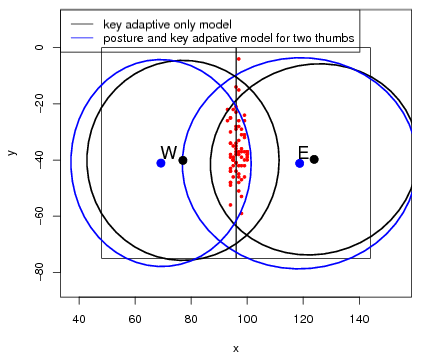
\includegraphics[width=1\columnwidth]{figures/key-posture-ellipse.png}
  \caption{Comparison of Gaussian distributions.}
  \label{fig:e-w-ellipses-1}
\end{figure}

Our cross-validation analysis, off-device simulation and on-device simulation based
on data collected from 32 users show
that both posture and individual adaptation can improve the probability estimation. For posture 
adaptation, with perfect posture information, the error reduction is 12.03\%; for individual adaptation, with perfect
intended key information, the error reduction is 14.68\%. The combination of the two 
can potentially give further improvement. 

In the real world application, posture classification and user adaptation need to be
online an in realtime, and these can introduce errors. For instance, when the user switches posture,
the adapted spatial model may in fact give less accurate estimate if the posture classification
is wrong. For individual adaptation, we need enough data points to build
an accurate Gaussian model because the points we use to update a model may not be accurate. 
To mitigate these problem and consider all the different criteria of adaptation, we 
introduce a hierarchical spatial models with back-offs for touchscreen keyboards.  
This means that if the confidence of the posture classification is not high or the Gaussian model for a particular user, posture and key combination is 
not valid, we back-off to a more general model that only adapts to two, one or even none of 
the criterion. 

The paper makes the following contributions. First
we propose a hierarchical adaptive spatial model that combines different
ways of spatial adaptation to improve the accuracy of key probability estimation, and provides seamless back-offs when necessary.
Second we compare the effectiveness of different adaptive strategies.
The result provides a guidance on the priority of the adaptation strategies to use during 
back-off. Third We develop a posture classification method that gives 86.4\% accuracy in
classifying each touch point into either one-finger or two-thumb input. Finally, we 
combined posture classification and the hierachcial adaptive spatial model in off-device and 
on-device simulation and showed that posture and individual adapation can improve the key probability
estimation.

\section{Related Work}
There is a body of active research on using spatial model, language model, or a combination
of the two to improve text entry accuracy on a soft touchscreen keyboard. For examples, 
Al Faraj et al. \cite{AlFaraj:2009} and Magnien et al. \cite{Magnien:2004} both use
visual highlight of the next possible keys to aid users' typing. Their predictions of the next keys are
based on language model. As our focus is on the 
spatial model, we will also mainly look at the related work in this aspect.    

Kristensson et al. \cite{Kristensson:2005} propose a geometric pattern matching technique to improve 
stylus input accuracy. They treat the touch points on a stylus keyboard as geometric pattern. 
This pattern is then matched agains patterns formed by 
the letter key center positions of legitimate words in a lexicon. Similar to this approach,
they also develop a gesture-based stylus input method where users only need to stroke between the keys \cite{Kristensson:2004}.
Their approaches essentially use a combination of spatial model and language model. However, 
their spatial model is not adaptive as they treat every key to have 0 offsets from 
the key center. While our focus is on tapping input, the same adaptive spatial model
can be applied to the gesture-based input.

In terms of spatial model that is adaptive to the keys (i.e. each key has its own model instead of
sharing the same model), Goodman et al. \cite{Goodman:2002} use bivariate Gaussian distribution with means, and
covariance matrices computed separately for each key in their study on stylus input. Zhai et al. \cite{Zhai:2002} also show that
the hit points for each key on a Metropolis keyboard \cite{Zhai:2000} are normally distributed and 
the centers of the distributions shift to different directions depending on the positions of
the keys. In their relative keyboard input system, Rashid et al. \cite{Rashid:2008} also use a different bivariate
Gaussian for each key. The error rate of their system is high because the lack of 
a priroi determined keyboard position.

Building on \cite{Goodman:2002}, Gunawardana et al. \cite{Gunawardana:2010} use restricted bivariate Gaussian
models in their anchored key-target resizing method. Key-target resizing means dynamically
adjusting the underlying target areas of the keys based on their probabilities. The probabilities can 
be a combination of spatial model probabilities and language model probabilities.
They argue that overly aggressive
key-target resizing can sometimes prevent users from their desired text, and hence violate
users' expection about keyboard functionality. They ensure that touch points within
the anchor area of a key is always detected as that key irrespective to the lanuage model.

There is also a number of research related to personal adaptation. 
Rudchenko et al. \cite{Rudchenko:2011}
developed a text entry game called \textit{Text Text Revolution} that provides 
targeting words for users to type to improve their typing experience. As a side effect,
the game also generates labeled touch point data which can be used as
training data to build the spatial models. They explore the effect of personal adaptation
by using the touch points from the first 10 rounds (about 250 characters and 50 words per round) of each 
participant's game play to build the personalized model for each key, and simulating the key detection
process for the second 10 rounds. Their result shows that with key-target resizing base on
spatial model probabililty only and using the training data from all the users combined
gives an error reduction of 18.9\% over no key-target resizing. When using personalized
key-target resizing, there is a further 2.84\% error reduction over non-personalized key-target resizing.
Their results show the benefit of individual adaptation in an ideal condition where the 
intended key is known. In the real world application, the keys users intend to hit are unknown and
can only be inferred base on the current spatial and language models. In our simulation, we assume the 
intended keys are unknown, and hence the result may be closer to the real world situaton. 

Findlater et al. \cite{Findlater:2012} uses a J48 classifier to classify
each key-press to specific keys for ten-finger touchscreen typing. They
focuses on individual adaptation and suggests that personalized touch keyboard
which adapts its underlying key-press classification models to the users can improve typing speed.  
In their user study, each key was intially seeded from 5 points sampled from
a bibariate Gaussian distribution, and the keyboard only started adatping
after a minimum of 10 points were collected from key presses. They did not
give reason about the choice of theses numbers, and did not explore the
effect of these numbers with respect to accuracy. 

The study from Findlater et al. also shows that displaying the adaptation visually can hinder
the performance. This result is also supported by the findings from Himberg et al. \cite{Himberg:2003} who 
studied vidually adaptive nine-key numeric keypads based on individuals.  

The key and individual adaptive methods mention earlier all assume that users' input posture
remain the same. We observe that the same individual may change hand posture even on the same device. 
The study from Azenkot and Zhai [1] shows that there are significant differences 
in typing speed and error rate between two-thumb input posture and one-finger 
input posture. More importantly, the horizontal and vertical offsets are 
different for each key and posture combinations. The most difference is that the for
one-finger input, the touch points for the keys on the left side of the keyboard tend to
shit to the right from the center of the target key whereas for two-thumb, the shift for those
keys are to the left. This suggests that automatic posture detection and posture
adaptive spatial model can potentially improve key detection accuracy. They listed those observations but
did not further investigate how posture adpatation can be implemented and how it can atually
affect key detection accuracy.

Finally, various researchers have explored other dimensions to improve the overall
text input experience on touchscreen keyboard. One dimesion is using hardware
augmentations to provide vibro-tactile feedback \cite{Hoggan:2008, Brewster:2007}. 
Another dimension is using alternative keyboard layouts that are optimized for typing speed (wpm)
based on Fitts' law and character level digraph frequencies \cite{Zhai:2000, MacKenzie:1999}.
These dimensions are orthogonal to the lanuguage and the spatial models, and can be potentially 
combined together to further increase the input accuracy and speed.

\section{Hierarchical Adaptive Spatial Models}
To incorporate different strategies of adaptations, we propose a hierarchical
spatial model consisting of a number of sub-models.
The entire model can be viewed as a hierarchy of sub-models in different
“orders” (Figure. \ref{fig:hierarchy}).

\begin{figure}[tb]
  \centering
  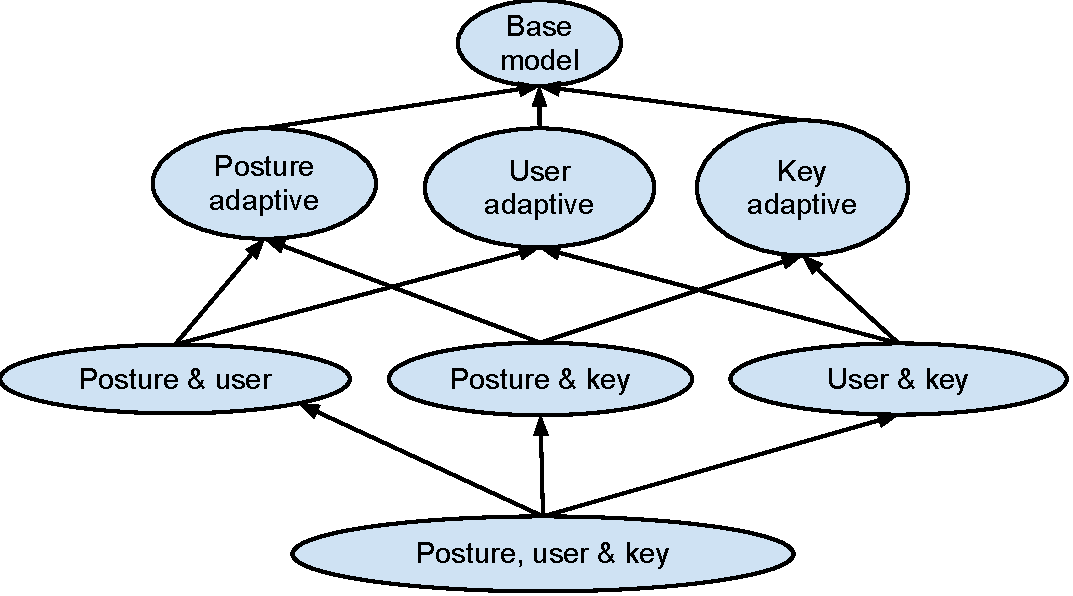
\includegraphics[width=1\columnwidth]{figures/hierarchical-spatial-model.pdf}
  \caption{Hierarchical spatial models}
  \label{fig:hierarchy}
\end{figure}

The zeroth order is the base model which is key, person, and posture
independent. This is the most general model combining all data together. The
higher order models consist of a combination of spatial models that adapt to hand 
posture (e.g. one finger, two thumbs, or ten fingers on tablets) , key or 
bi-letters (e.g. "h/t” where the current target letter is the “h” key and the 
previous letter is “t”), and the individual user. 

The higher the order of the sub-model, the more data is required to build the model because
the model is more complex with more parameters. This means that each combination of the 
conditions needs sufficient number of samples to build a reliable model. Each 
such sub-model would only become active when its reliability passes a set 
threshold (e.g. more than 100 points had been collected); otherwise these models
 that are still “growing” but in “dormant” mode.

\section{Comparison of Spatial Models}
We compare key detection error rate with different models to analyze their
relative effectiveness (Table \ref{tab:comparison}). This can inform us the order of the
back-off models to use when there is not enough data for higher order models.
10-fold cross validation is used, and the training and testing data sets have
different sets of users.

\begin{table} [tb]
  \centering
  \begin{tabular}{|l|c|}
    \hline
    \tabhead{Spatial model} &
    \multicolumn{1}{|p{0.2\columnwidth}|}{\centering\tabhead{Key detection
    error rate}} \\
    \hline
    Distance from the center of the keys & 7.976\% \\
    \hline
    \multicolumn{1}{|p{0.7\columnwidth}|}{Base model (same Gaussian model for
    all the keys with a full covariance matrix)} & 7.853\% \\
    \hline
    Key adaptive model  & 8.023\% \\
    \hline
    Posture and key adaptive model & 7.058\% \\
    \hline
    User and key adaptive model  & 6.845\% \\
    \hline
  \end{tabular}
  \caption{Comparison of key detection accuracy (no language model) with
  different spatial models using 10-fold cross validation.}
  \label{tab:comparison}
\end{table}

Evaluation is based on a data set collected from an earlier study of 32
participants. Users were given target phrases to type on a Nexus S phone. The
details of the study can be found in this paper \cite{Azenkot:2012}. This was a between-user
study in which each user used one posture to type.
We remove the data from 2 left-handed users in our analysis, and are left with
data from 9 users with one-index-finger input, 11 users with one-thumb input and
10 users with two-thumb input.  In our analysis, we combine the data from index finger input
and one-thumb input togetehr. So two postures are considered here: one-finger versus two-thumb. We also filtered out points that are 1.5 times
the height of the key away from the center of the target key. Note that the ratio
of the number of users using one-finger input to that using two-thumb input is kept the same
for the training and testing data sets throughout the cross-validation.

The simpliest base model can have a Gaussian distribution with 0 x and y
mean offsets and the same spherical covariance matrix for all the keys. Key
detection based on this model is essentially choosing the key that has the shortest Euclidean distance from the tapping coordinates. 
One step beyond this is to have a full covriance matrix trained from the
training data, but still using the same Gaussian model for each key.

\subsection{Key Adaptation}
A basic key adaptive model is building a bivariate Gaussian model for each key 
using data from many different users. Then the key detection process involves 
choosing the key whose Gaussian model gives the highest probability for the 
given (x, y) tapping coordinates. When this is combined with posture and 
individual adaptation, more specialized Gaussian models are built for each key.

The difference in key detection accuracy between using the base model only and
the key adaptive model is not big. It is even surprising that key adaptive model
gives slightly lower accuracy. A closer look at the data shows that the most number of error occurs between
``E'' and ``W''. Because there are more one-finger input users in the data set, the 
Gaussian models built for ``E'' and ``W'' have right horizontal offsets. However, for the two thumb input, 
there is usually a left horizontal offsets. Hence there are more errors for tow-thumb input.

This suggests that key adpative model may not be always effectivce unless we have enough data and a balanced
number of postures in the training data. But since the key adaptive model can be trained offline by collecting data from a 
large number of users, this shows that it can be used as the basic backup model once we collect enough data. 

\subsection{Posture Adaptation}
Key adaptation becomes more effective when combined with posture adaptation. There can be different levels of
complexy for posture adapation. For the most complex one, we can build two models for each key for the 
two input posture; or we can do posture adaptation for a certain number of keys. The best result is obtained when we only do 
posture adaptation for the keys on the left side. The error rate for postur and key adaption shown in the table is 
based on posture adaptation for the keys on the left side. Note the choice of this set of keys
is not arbitrary. As observed by Azenkot et al. \cite{Azenkot:2012}, the difference in horizontal
offsets of the touch points from different postures are most prominent for the keys on the
left set (Note that for left-handed users, the reverse is probably true). 
In addition, the analysis of variance based on the tapping coordinates in the data set shows
that, for different postures, there are significant differences in the means of
the $x$ coordinate for the keys on the left side of the keyboard and the
``space'' key ($p < 0.05$). 

There is 12.03\% reduction in error rate compared to key adaptation only. Two
sample one sided paired t-test shows that the improvement in accuracy is
significant when we use posture and key adaptation versus key adaptation only (t (29) = -2.4421, p = 0.01).

Figure \ref{fig:key-boundary} shows the comparison of effective areas of the keys
with different spatial models. Each colored area presents the region such that if the
user tap in that region, the underlying spatial model will classify that key with the 
corresponding key label. Note how the key areas for the left-side keys shift to the left
for two-thumb input and shift slightly to the right for one-finger input. The difference in 
the effective key areas is the same concept as key-target resizing mentioned in \cite{Rudchenko:2011, Gunawardana:2010}.

\begin{figure}[tb]
	\centering
	\subfigure[Key adaptive model]{
    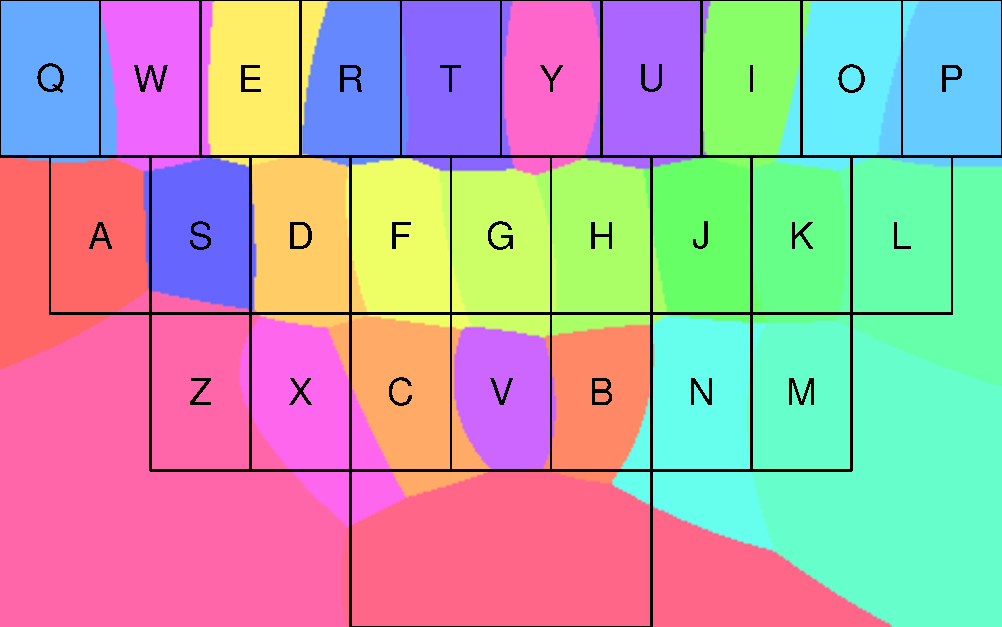
\includegraphics[width=0.47\columnwidth]{figures/key-model.pdf}
    \label{fig:subfig1}
	} ~
	\subfigure[Posture and key adaptive model for one-finger input]{
    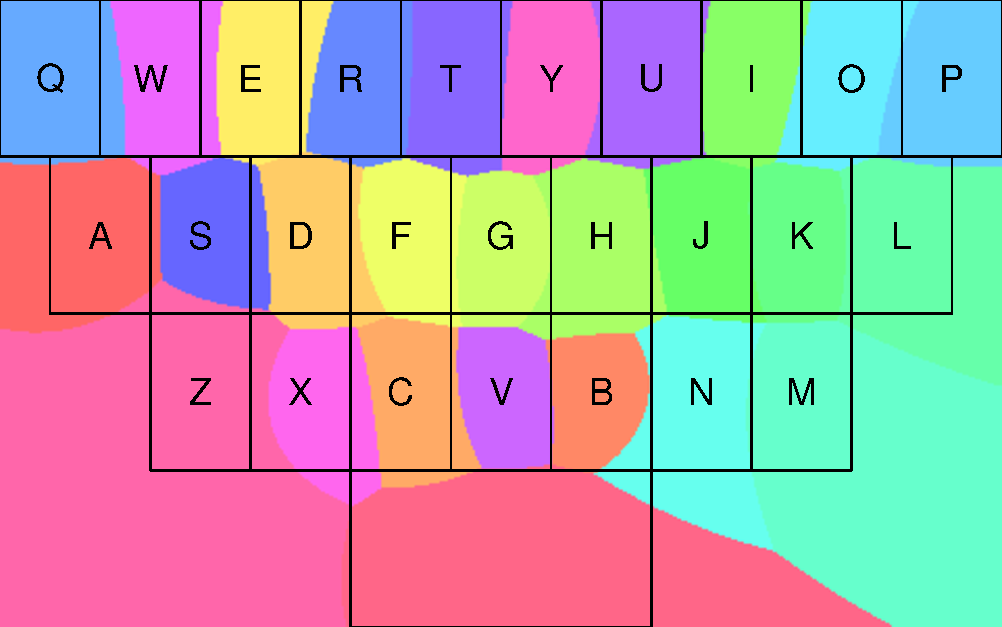
\includegraphics[width=0.47\columnwidth]{figures/posture-t.pdf}
    \label{fig:subfig2}
	}
	\subfigure[Posture and key adaptive model for two-thumb input]{
    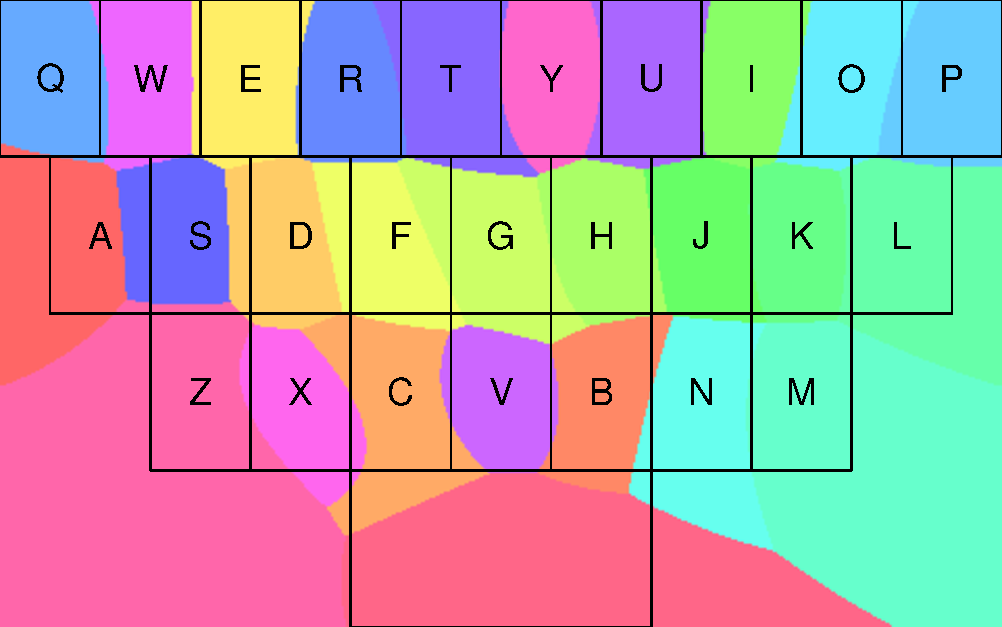
\includegraphics[width=0.47\columnwidth]{figures/posture-tt.pdf}
    \label{fig:subfig3}
	}
	\caption{Comparison of effective key areas with different spatial models}
	\label{fig:key-boundary}
\end{figure}

The accuracy is based on perfect knowledge of the posture which represents an
upper bound for posture adaptation for these data sets. In the actual 
implementation, the posture model can be turned on when we have high enough 
confidence about the posture classification.

\subsection{Individual Adaptation}
The user and key adaptive model gives the lowest error rate compared to other models. 
This suggests that user and key adaptation can have higher priority in the hierarchy and during
backoff. 

For user and key adaptation, for each fold, we use 90\% of the users to train the
combined back-off key models. Then for each of the 10\% testing users,  a
fraction k of the data for each key is used to train the user adaptive key
models. The accuracy of these data points are tested on the combined key models.
The remaining 50\% of the data for each user are tested on the user adaptive 
models together with the combined model for backup. The backup is used when 
there is not enough data for certain key (we used 10 data points) to build the 
Gaussian model. In this analysis, $k$ is set to be 50\%.

However, it should also be noted that we need enough data points to build an
accurate model for each key for each individual. Figure~\ref{fig:user-adapt}
shows how key detection accuracy changes as the number of points used to build
the personalized model for key 'E' increases. For the user adaptation to be
effective, we should use it when the accuracy is greater than then non-user
adaptive model. As our dataset has limited number of keys
pressed from each user, we only shows the trend when the nubmer is 70. However,
the figure still shows a general trend, and suggests that a number in the order
of a hundred is probably a good nubmer. When we do not have enough data for the
user, we can use posture and key adaptation.

\begin{figure}[tb]
  \centering
  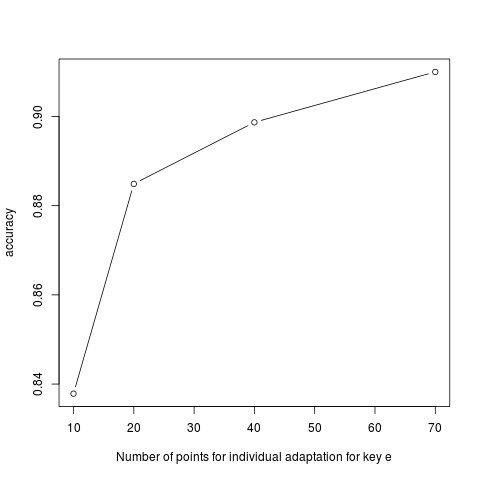
\includegraphics[width=1\columnwidth]{figures/user-adapt-e.png}
  \caption{Tapping points data from input on a Nexus S phone.}
  \label{fig:user-adapt}
\end{figure}

The key spatial model can also be more specialized to include bi-letter patterns
that occur frequently, for instances, h followed by e, t followed by h etc. 
Figure 2 shows the (x, y) coordinates of the tapping points for letter “e” from 
one of our data sets, and the 0.95 confidence ellipses of the Gaussian models 
for different conditions. The plot shows that when we combine data for all the 
posture together, the distribution of points for “e” after “h” is very slightly 
different from that of all “e”. But if we look at “e” after “h” for one-finger input (cyan color), the difference is bigger. Another point to note is that, since these are highly frequent patterns, even a small improvement in detecting these keys based on these more specialized models may give a bigger improvement in the overall key detection accuracy.


Figure 2. Comparison of Gaussian models (0.95 confidence ellipses) for letter “e”

\section{Input Hand Posture Classification}\label{sec:posture-classification}
To incorporate posture adaptive spatial models, we developed a binary hand-posture classifier 
that constantly returns an estimate of the user's current posture (two-thumb or one-finger input).
Let $\mathcal{Y} = \{\text{one-finger}, \text{two-thumb}\}$ be the set of posture
class labels. We describe in detail the classification function that maps input from the
touch points to $\mathcal{Y}$.

Our method of hand-posture classification is based on Fitts’ law which states that the time (T) required to move to a target is a function of the distance (D) to the target and the size (W) of the target (Equation 1).
\begin{align}
T = a + b\log_2(1 + \frac{D}{W})
\end{align}                                                  
The insight here is that we expect the one-finger input posture follows this law,  but two-thumbs input may not. For example, when the user types “al”, it takes longer time to type using one finger because the distance between these two keys are large, but with two thumb, it can be very fast because she can use the left thumb to type “a” and the right thumb for “l”.

\begin{figure}[tb]
  \centering
  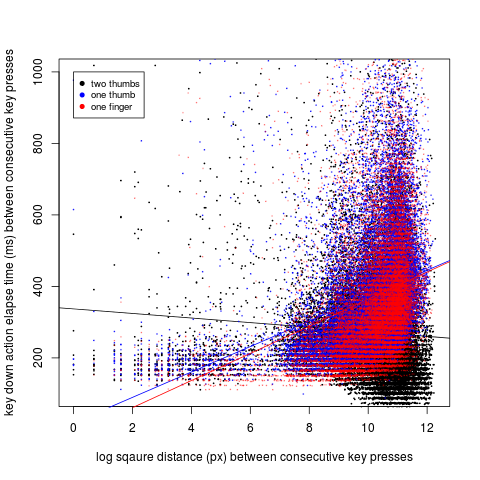
\includegraphics[width=1\columnwidth]{figures/time-distance.png}
  \caption{Tapping points data from input on a Nexus S phone.}
  \label{fig:time-distance}
\end{figure}

Figure. \ref{fig:time-distance} shows the relationship between the time elapsed 
and the log square distance travelled between consecutive key presses. We can
see that for the one-finger input (blue and red points), the time taken
increases with distance whereas for the two-thumb input, there is no obvious
trend. The difference is more significant when the log square distance (natural
log) is greater than 10 px.

Based on this finding, we include the time elapsed and the log square distance
between two consecutive key presses as the features for the posture classifier. 
To account for individual typing speed differences, we also use normalized time 
elapsed between consecutive key presses as the third feature. It is calculated according the following equation:

\begin{align}
\text{Normalized time elapsed} = \frac{\text{time elapsed}}{\text{average time
elapsed for the last 10 key presses}}
\end{align}

We train a SVM classifier with these 3 features for consecutive tap points that 
are on different sides of the keyboard and whose log square distance is at least
10px. We use 70\% of the data for training and 30\% of the
data for testing. The users in the training and testing data sets are different.

The Pepper (84292 filtered data points) data sets we use consist tapping points 
from different users with different postures. The classification accuracy from
the single tap classifier for keys with previous key on the different sides of
the keyboard 83.559\% (11090/13272).

The single tap classifier gives a probability score $p_y^{\text{single}}$ for each posture for touch
points whose previous key tap is on the different side of the keyboard. Note that
$\displaystyle\sum_{y \in \mathcal{Y}}p_y^{\text{single}} = 1$.
 
In order to classify every key tap and assuming the user does not change posture 
rapidly, we look at a sliding time window of 10 key taps (about 2 words). For 
each time window, we use another SVM classifier with the following features:
\begin{enumerate}
\item Correlation between time elapsed and log distance (this feature has the
advantage of being speed independent) (see Figure. \ref{fig:boxplot}).
\item The average probability score for each tap to be one-finger input.
\item The average probability score for each tap to be two-thumb input.
\item The average number of taps classified as one-finger input.
\item The average number of taps classified as two-thumb input.
\end{enumerate}
The history of the touch points are cleared for every new typing session.
The choice of the size of the sliding window represnts a trade-off between the 
accuracy of the classification and how responsive the system is when the user
changes posture. We found that the assumption that the user does not change posture
often within 2 words is reasonable, but more work can be done to investigate this
aspect, and even to test with a window size of 1 (i.e. not 
looking at the history).

The sliding time window classifier gives a final probability score $p_y$ for posture
$y$ for each touch point. Again $\displaystyle\sum_{y\in \mathcal{Y}}p_y = 1$. To evaluate the classification accuracy, we set the the
classified posture to be $y$ if $p_y > 0.5$. With this, the overall classification 
accuracy for each touch point with a sliding time window
is 86.401\% (23128/26769).

Because of the sliding window approach, the posture for the first few touch points  
for each new session is unknown. In this case, we can use a lower order spatial 
model (key adaptive or base model). Furthermore  we can turn on the posture 
adaptive spatial model only when the probability score for one posture is much 
higher than the other.

\begin{figure}[tb]
  \centering
  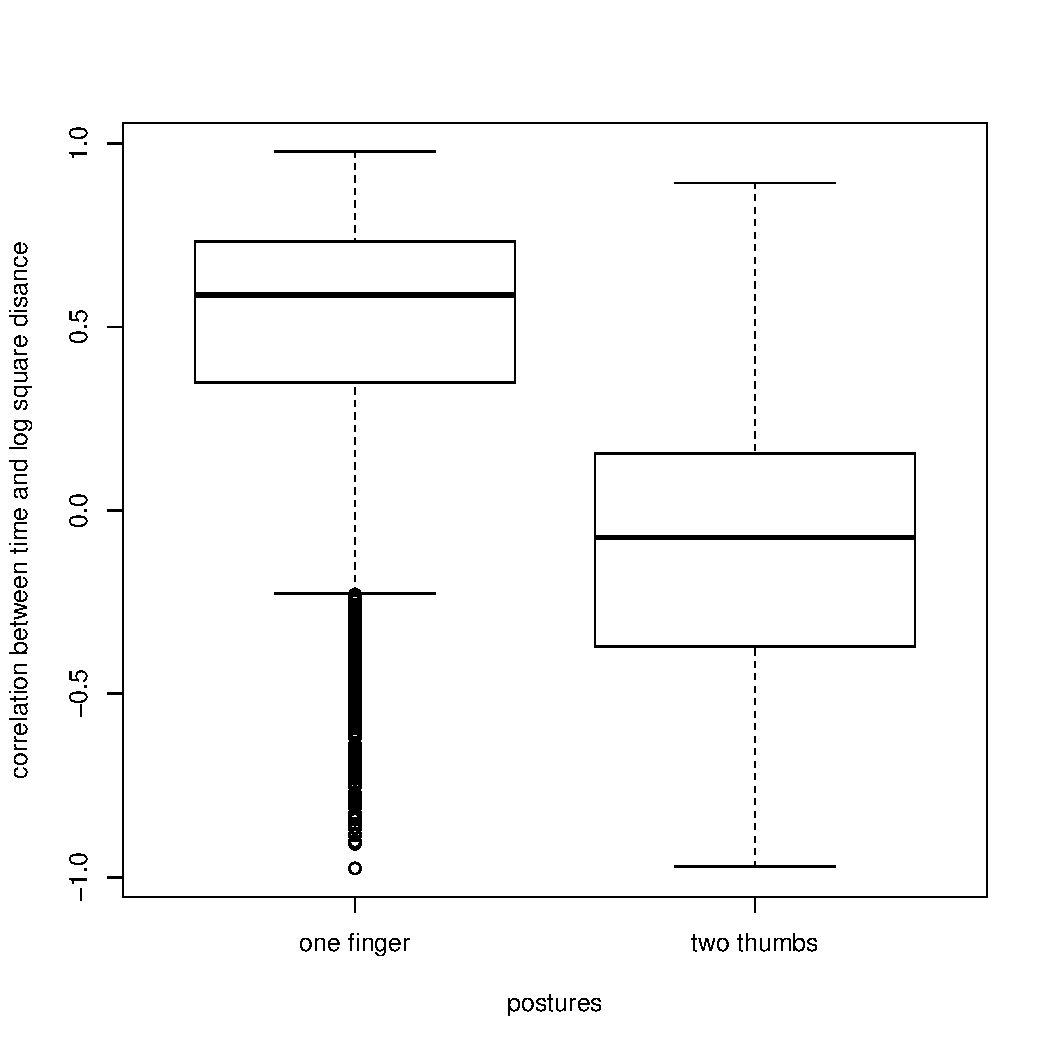
\includegraphics[width=1\columnwidth]{figures/boxplot.pdf}
  \caption{Correlation between time elapsed and log square distance between
  consecutive key presses for every 10 keys. There is a stronger correlation for
  one- finger input than that for two-thumb input.}
  \label{fig:boxplot}
\end{figure}

\section{Key detection process}\label{sec:key-detection-process}
In the detection process, a higher order more specialized model is used if it
meets a set of conditions such as a particular posture mode is detected with high 
confidence and the corresponding model (e.g. key 'E' for user A using
one-finger) is available (live, matured).
Otherwise we back off to a lower order model, all the way to a base model which 
is key, individual and posture independent if necessary. The order of the
backoff process, and the priority of the model at the same level to use can be
design choice, but our previous section also gives a guidance and suggestion on
how to determine the order.

In terms of implementation, this detection process also fits nicely with the
Chain of Responsibility desgin pattern.
Figure~{fig:chain-of-responsibility} shows a simplified version of an object
diagram showing the interaction between various models. Each higher model can
have a reference or references to lower order models. When given a pair of touch
point coordinates, the system queries the highest order model for a Gaussian
model, if it is not present, the higher model calls the lower model, and the
query propagates until a Gaussian model is found.

\begin{figure}[tb]
  \centering
  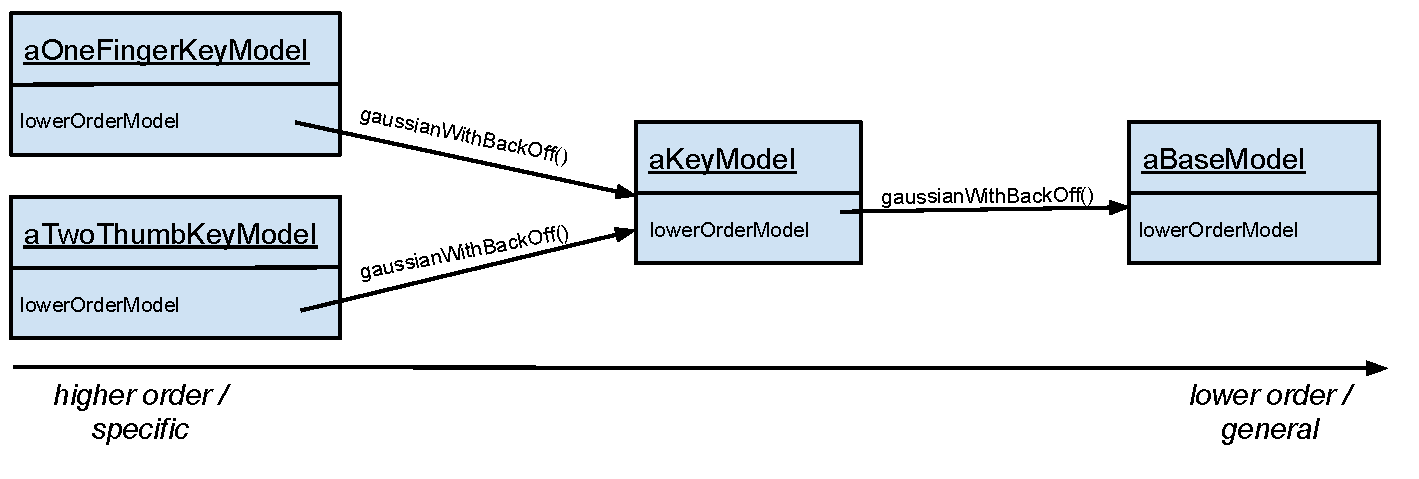
\includegraphics[width=1\columnwidth]{figures/chain-of-responsibility.pdf}
  \caption{An object diagrame showing the interaction between higher and lower
  order spatial models.}
  \label{fig:chain-of-reponsibility}
\end{figure}

\section{Implementation and Simulation}
We implemented a prototype similar to what is described in
Section~\ref{sec:key-detection-process}, also combining online posture
classification. We did a simulation using 20 users' data for training
both the posture classifier and spatial model, and tested on the other 10 users' 
data. The percentages of one finger input and two thumbs input postures are the same in both the training and testing data sets.

\subsection{Off-device Simulation}
We did off-device simulation to compare
key detection error rate using different spatial models without language model.
Table~\ref{tab:off-device} shows the results.

\begin{table}[tb]
  \centering
  \begin{tabularx}{\columnwidth}{|X|c|}
  \hline
  \tabhead{Spatial model} & \tabhead{Error rate} \\
  \hline
  \multicolumn{1}{|p{0.7\columnwidth}|}{Base model (same Gaussian model for
    all the keys with a full covariance matrix)} & 8.641\% \\
  \hline
  Key adaptive model & 8.708\% \\
  \hline
  Posture and key adaptive model & 8.394\% \\
  \hline
  User and key adaptive model & 8.256\% \\
  \hline
  User and key adaptive model  & 7.621\%
  \\
  \hline
  User, posture and key adaptive model &  7.498\%
  \\
  \hline
  \end{tabularx}
  \caption{Off device simulation result}
  \label{tab:off-device}
\end{table}

\subsubsection{Posture Adaptation}
The posture and key adaptive model shown here uses the posture classification
method described in Section~\ref{sec:posture-classification}. As a result, the
key detction error rate for using this model is compounded with the posture
classification error rate as well. 

An error in posture classification will lead to the choice of wrong spatial model,
and hence adversely affect the key detection accuracy. To mitigate this problem, we
adopt a conservative approach, and only use posture adapation when the confidence of
the classification result is high.

The confidence of the classification is reflected by the pair of probability 
scores $(p_{\text{one-finger}}, p_{\text{two-thumb}})$ returned by the classifier. 
We can set a threshold $T_{\text{posture}}$ such that the input posture is classified
as $y$ only if $P_y \ge T_{\text{posture}}$ . Otherwise the posture is treated as
unknown and we back-off to a lower order spatial model.

There is also a trade-off in setting the threshold $T_{\text{posture}}$. The higer
 $T_{\text{posture}}$ is, the fewer the number of errors there are in posture classification, but at the same time,
 the fewer the number of touch point postures will be classified. In other words, 
 more touch points will be classified as from unknown posture and no posture adaptation 
 is used for these touch points. Figure~\ref{fig:posture-confidence} shows how
 the accuracy of key detection changes as the confidence threshold increases. It 
 shows that there is an optimal level of the threshold beyond which the accuracy
 decreases because we are no longer taking the advantage of posture adaptation.

\begin{figure}[tb]
 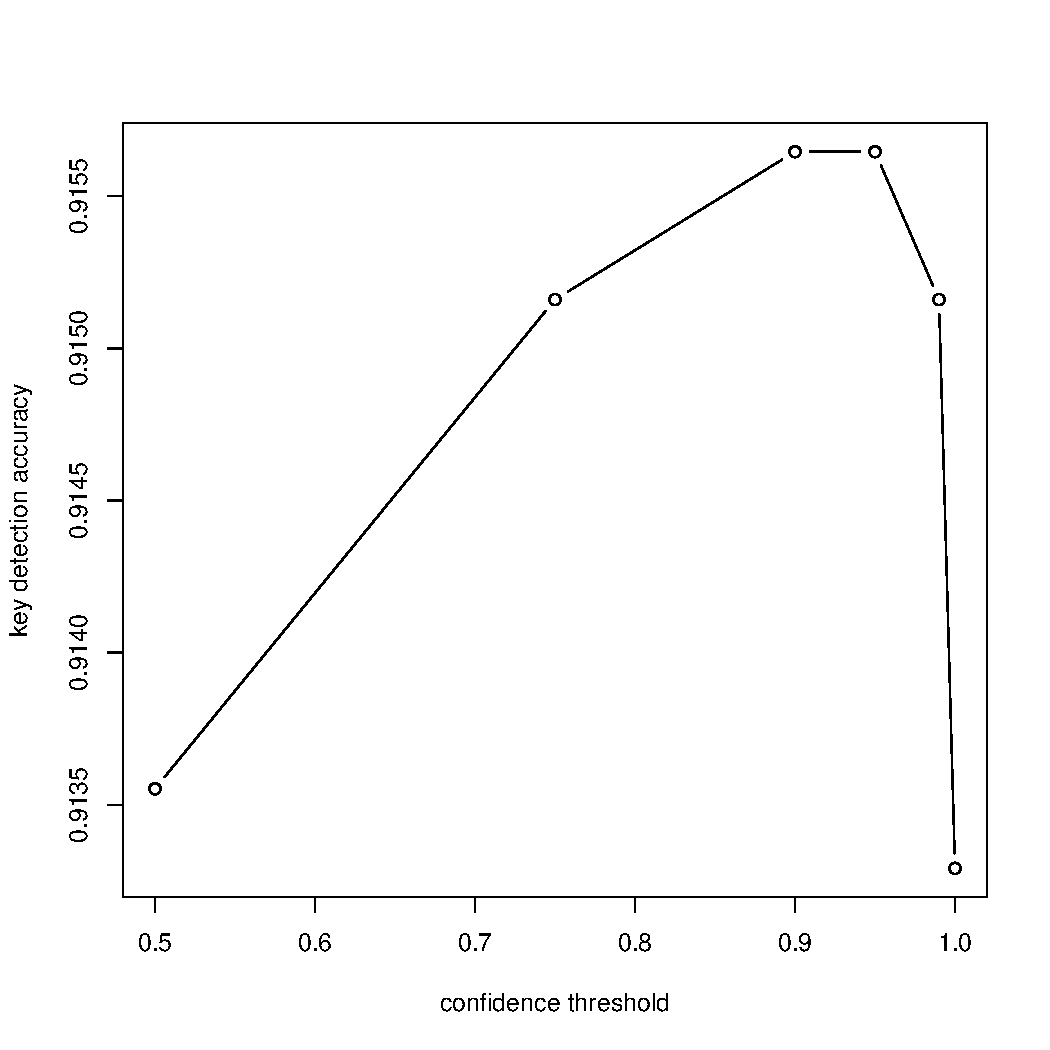
\includegraphics[width=1\columnwidth]{figures/posture-confidence.pdf}
  \caption{Graph showing how key detection accuracy changes with confidence
  threshold for posture classification.}
  \label{fig:posture-confidence}
\end{figure}

The error rate when using posture and key adaptive model shown in Table~\ref{tab:off-device}
is obtained by setting $T_{\text{posture}} = 0.94$.

To further investigate the effect of posture adaptation, we looked at the detection
errors when using key adaptive model only as compared to when using posture and key adaptive model.
Figure~\ref{fig:confusion-matrices} shows the confusion matrices from the key detection
simulation for the key adaptive model and the posture and key adaptive model. Each 
confusion matrix is a representation of the key detection errors. The row labels are
the target keys, and the column labels are the predicted keys. The color of the cells
represnts the number of errors for a particular pair of confusion. The more red the color,
the greater the number of errors. Figure~\ref{fig:error-key} and \ref{fig:error-posture}
shows errors when using key adaptive model and posture and key adaptive model respectively.
The most frequent mistake for both models are ``A'' and ``S'' confusion. Figure~\ref{fig:error-key-posture}
and \ref{fig:error-posture-key} shows errors in one of the models but not in the other one.
We can see that when using posture and key adaptive errors we also incurr errors
that are not present when using key adatpve model alone. However the number of these
errors are much smaller compared to the errors corrected.

\begin{figure*}[tb]
	\centering
	\subfigure[Errors when using key adaptive model]{
    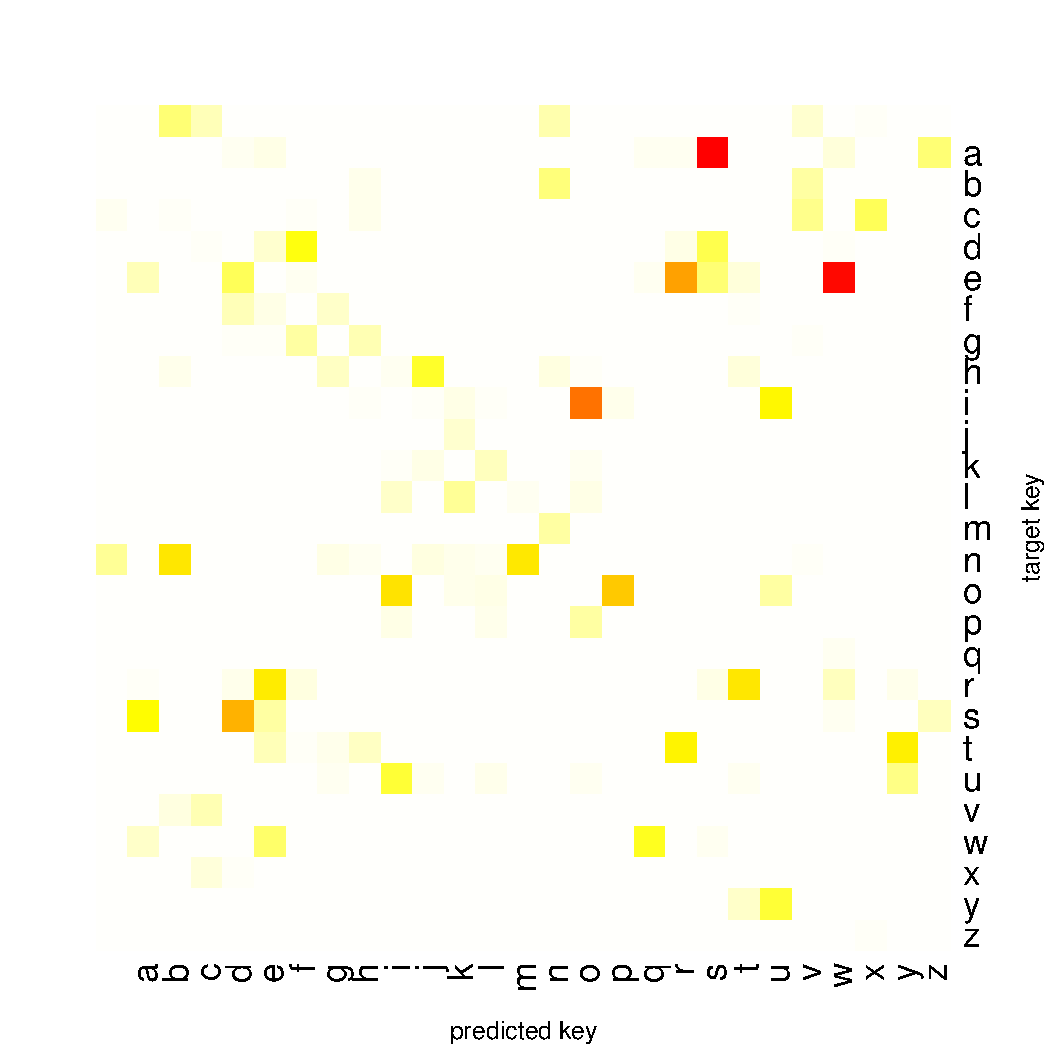
\includegraphics[width=0.49\columnwidth]{figures/sim-result-1.pdf}
    \label{fig:error-key}
	} 
	\subfigure[Errors when using posture and key adaptive model]{
    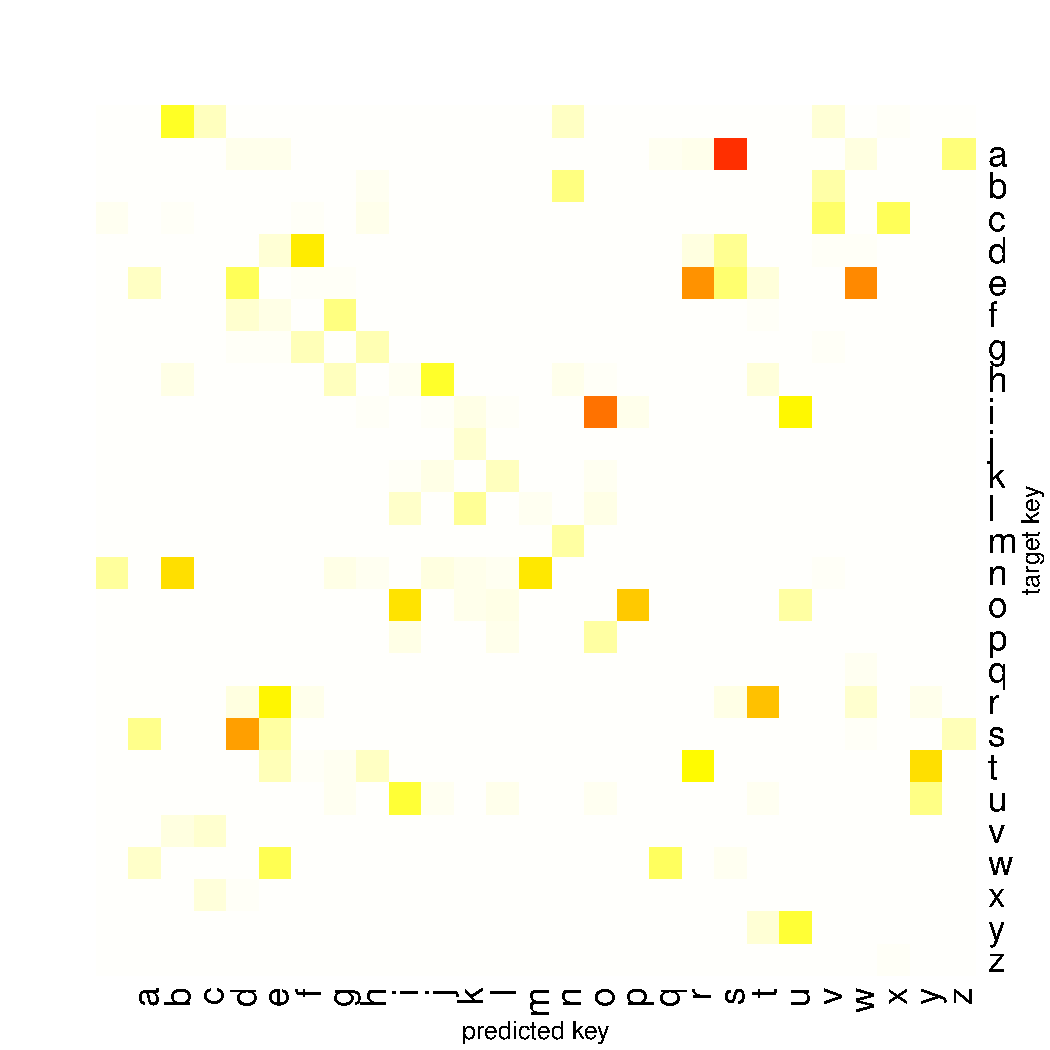
\includegraphics[width=0.49\columnwidth]{figures/sim-result-2.pdf}
    \label{fig:error-posture}
	}
	\subfigure[Errors when using key adaptive model but not when using posture and key
	adaptive model]{
    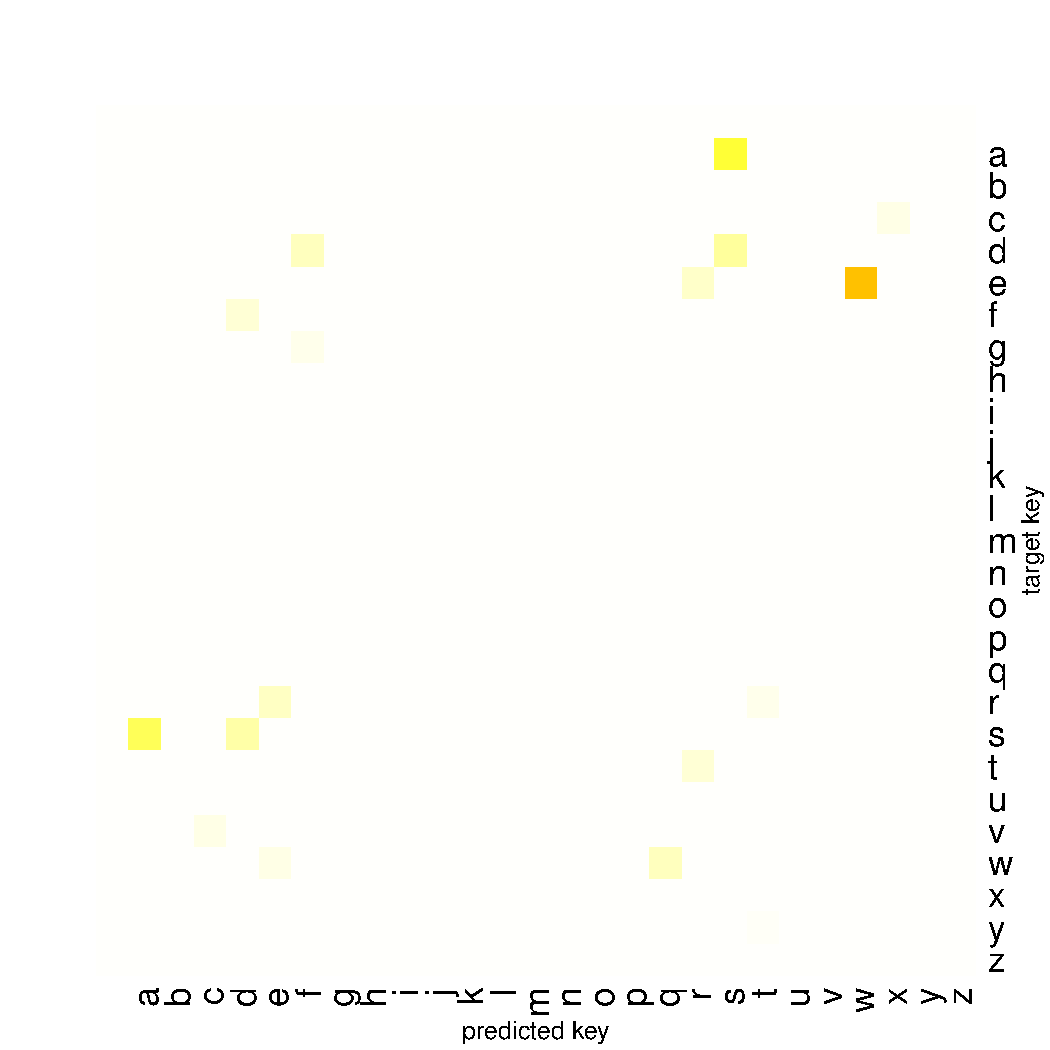
\includegraphics[width=0.49\columnwidth]{figures/sim-result-1-2.pdf}
    \label{fig:error-key-posture}
	}
	\subfigure[ErrorS when using posture and key adaptive model but not when using key
  adaptive model]{
    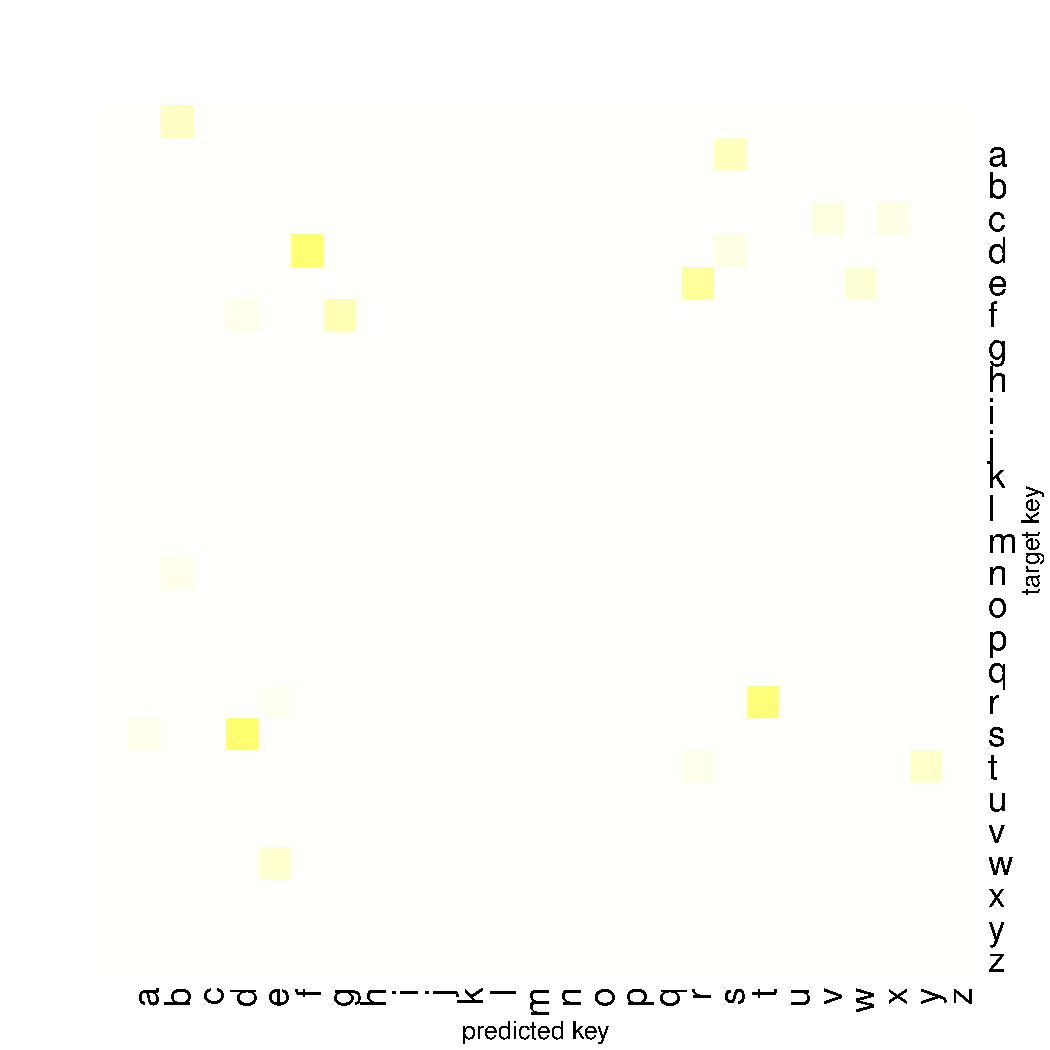
\includegraphics[width=0.49\columnwidth]{figures/sim-result-2-1.pdf}
    \label{fig:error-posture-key}
	}
	\caption{Confusion matrices for different
	spatial models from off-device key detection simulation. The row labels are the
	target keys, and the column labels are the predicted keys.}
	\label{fig:confusion-matrices}
\end{figure*}

From the figure, we also observe that the most number of corrections by using posture
and key adaptive model is for the ``E'' and ``W'' pair. Figure~\ref{fig:e-w-ellipses}
shows a closer look at the Gaussian models for the two keys for the different
spatial models. Each ellipse represents the 0.95 confidence ellipse of the Gaussian model built 
based on a set of touch points.
Each black ellipse is based on the touch points intended for either ``W'' or ``E''. 
For the blue ellipses, they are drawn similarly but only touch points from two-thumb input
are included. The red points are the touch points that are detected as ``W'' when the target
key is ``E'' when using the key adaptive model. We can see the black ellipses are shifted
slightly to the right probably because there are more touch points from one-finger input in the training
data. The causes the touch points on either sides of the boundary between ``W'' and 
``E'' to be mis-classified as ``W''. However, the ellipses based on the posture and key
adpative model for the two-thumb input shifts to the left slightly, and this changes
the classification of those boundary points to ``E'' correctly.

\begin{figure}[tb]
 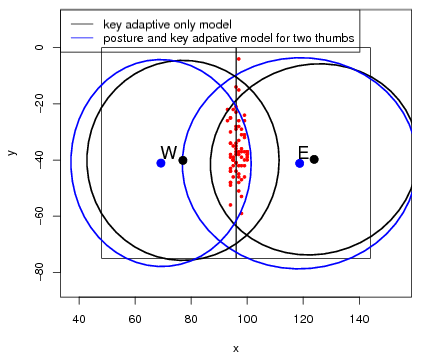
\includegraphics[width=1\columnwidth]{figures/key-posture-ellipse.png}
  \caption{Comparison of Gaussian distributions.}
  \label{fig:e-w-ellipses}
\end{figure}

\subsubsection{Individual Adaptation}
For individal adaptive model, we set the minimum number of points needed to build the
Gaussian model for a particular key for a particular individual to be 50. This number is 
aslo affected by the limited amount of data we have because there are not many keys that has 
the number of touch points be greater than 50. Unlike the analysis using cross-validation
where we assume we know the target key perfectly, during online implementation, we can
only make the best possible guess about the user's target key and use the touch point
coordinates to update the Gaussian model for that particular key.

For every touch point, we compute the probability for each key given the underlying spatial model.
Then we use the $(x, y)$ coordinates of the touch point to upate the Gaussian model
for the most probable key. Updating the Gaussain model involves computing the running
average of the $x, y$ offsets from the center of the key and the covariance matrices. The counter 
for the number of points used for a particular key Gaussian is maintained so that we
know when a particular Gaussain model becomes valid, i.e. has enough data points.

When there is not enough data points, the system backs-off to a lower order model.
Here we can have a choice of whether backing-off to the posture and key adaptive model or 
to the key adaptive model. Backing-off to the posture and key adaptive model means
classify the user's current posture and use the corresponding posture and key model for key detection instead
of just using the key model which is posture independent. The last two rows in 
Table~\ref{tab:off-device} shows that there is also a slight more error reduction  in backing-off to
the posture and key adaptive model.

Note that because the data set we have is from a between-user study, we cannot look
at the effect of posture adaptation for each invidual, i.e., each indidual has two Gaussian models
for each posture and key combination.

\subsection{On-device Simulation with Language Model}
We also did a on-device simulation with language model auto-correction to see the
the effect of posture adaptation. The language model is the most basic one which
gives the same frequency for all the possible words in the dictionary. It does not
correct substition, insertion or deletion errors either.

During the decoding process, the system computes the cost of each touch point to
each key using the spatial model. The cost is the negative of the log probability of
the touch point given a Gaussian model for a certain key.

The metric we use is the mean word distance between the target phrase and the detected
phrase after auto correction across the users. The word distance is calcualted using 
edit distance at the word level. This means converting each phrase to a number coded
string (same phrase has the same numeric code), and then the edit distance is computed
between the two number strings. Substition, deletion and insertion all have the same
cost. The higher the score, the better the result.

With key adapative model only, the final score is 80.078; and with posture and key
adaptive model, the final score is 80.529. Table~\ref{tab:on-device} shows all the examples
in the test users where the detected phrases are correct when using posture and key adaptive spatial model, but
are wrong when using key adaptve only spatial model. We can see that in those examples,
the posture and key adpative model can correctly detect the phrases because it
correctly distinguish the neighboring keys between ``A'' and ``S'', ``S'' and ``D'',
``D'' and ``F'', ``F'' and ``G'', ``W'' and ``E''. 

There are also 4 cases there the detected phrases using key adaptive model is correct, but the ones
using posture and 

This shows that how the posture adaptive spatial model can potentially be combined 
with language model to give better auto correction result.

\begin{table*}[tb]
  \centering
  \begin{tabularx}{0.925\textwidth}{|l|l|l|l|}
  \hline
  \tabhead{Input posture} & \tabhead{Target phrase} & \tabhead{Detected phrase with key adaptive model} 
  & \multicolumn{1}{|p{0.526\columnwidth}|}{\tabhead{Detected pharase with posture and key adaptive model}}\\
  \hline
  two-thumb & the dreamers of dreams & the {\color{red}dream era} of dreams & the dreamers of dreams  \\
  \hline
  two-thumb & handicapped persons & {\color{red}handicap pes} persons & handicapped persons \\
  \hline
  two-thumb & she wears too much makeup & {\color{red}a he} wears too much makeup & she wears too much makeup \\
  \hline
  one-finger & my bare face in the wind & my bare face in the {\color{red}wins} & my bare face in the wind \\ 
  \hline
  two-thumb & a lie makes the nose grow & a lie {\color{red}ma kea} the nose grow & a lie makes the nose grow \\
  \hline 
  two-thumb & the bathroom is clean & the bathroom is {\color{red}cl wan} & the bathroom is clean \\
  \hline 
  two-thumb & travel at light speed & travel at light {\color{red}a peed} & travel at light speed \\ 
  \hline
  two-thumb & traveling requires fuel & {\color{red}travel inf require a} fuel & traveling requires fuel \\
  \hline 
  two-thumb & most golfers love the game & most {\color{red}gold ers} love the game & most golfers love the game \\ 
  \hline
  two-thumb & win first prize & win {\color{red}dir st} prize & win first prize \\ 
  \hline
  two-thumb & if at first you fail & if at {\color{red}dir st} you fail & if at first you fail \\ 
  \hline
  \end{tabularx}
  \caption{Examples of on-device simulation where the detected phrase is correct
  with posture and key adaptive spatial model and incorrect with key adaptive spatial
  model.}
  \label{tab:on-device}
\end{table*}


\section{Conclusion}

It is important that you write for the SIGCHI audience.  Please read
previous years' Proceedings to understand the writing style and
conventions that successful authors have used.  It is particularly
important that you state clearly what you have done, not merely what
you plan to do, and explain how your work is different from previously
published work, i.e., what is the unique contribution that your work
makes to the field?  Please consider what the reader will learn from
your submission, and how they will find your work useful.  If you
write with these questions in mind, your work is more likely to be
successful, both in being accepted into the Conference, and in
influencing the work of our field.

\section{Acknowledgments}

We thank all the volunteers, and all publications support
and staff, who wrote and provided helpful comments on previous
versions of this document.  Some of the references cited in this paper
are included for illustrative purposes only.  \textbf{Don't forget
to acknowledge funding sources as well}, so you don't wind up
having to correct it later.

% Balancing columns in a ref list is a bit of a pain because you
% either use a hack like flushend or balance, or manually insert
% a column break.  http://www.tex.ac.uk/cgi-bin/texfaq2html?label=balance
% multicols doesn't work because we're already in two-column mode,
% and flushend isn't awesome, so I choose balance.  See this
% for more info: http://cs.brown.edu/system/software/latex/doc/balance.pdf
%
% Note that in a perfect world balance wants to be in the first
% column of the last page.
%
% If balance doesn't work for you, you can remove that and
% hard-code a column break into the bbl file right before you
% submit:
%
% http://stackoverflow.com/questions/2149854/how-to-manually-equalize-columns-
% in-an-ieee-paper-if-using-bibtex
%
% Or, just remove \balance and give up on balancing the last page.
%
\balance

% If you want to use smaller typesetting for the reference list,
% uncomment the following line:
% \small
\bibliographystyle{acm-sigchi}
\bibliography{chi2013}
\end{document}
